%!TEX root = ../dissertation.tex
\chapter{Elaborazione dei dati di input} \label{elaborazione}

Per lo svolgimento del lavoro proposto viene utilizzato un set di dati costruito tramite un sensore 3D time-of-flight (noto anche come SoftKinetic DepthSense 325).
Senz3D è un prodotto realizzato in partnership con Creative, una videocamera con sensore di profondità che può essere installata su notebook e PC basati su architettura Intel e che, di fatto, opera come una sorta di Kinect per dispositivi Windows.
Il dispositivo ha sia una fotocamera RGB che un sensore di profondità Time-Of-Flight (ToF).
La risoluzione di profondità è 320 per 240 pixel, con un frame rate compreso tra 6 e 60. La funzione automatica di soglia della confidenza del sensore è stata utilizzata anche per ottenere una mappa di profondità iniziale migliore.

Il set di dati contiene gesti prodotti da quattro persone diverse, ciascuna eseguendo undici diversi gesti ripetuti trenta volte ciascuno, per un totale di 1320 campioni. Sono usati i dati delle prime tre persone per la fase di allenamento della rete neurale (quindi 990 campioni). Mentre i restanti 330, relativi agli undici gesti dell'ultima persona, vengono utilizzati per la fase di test.
Per ogni campione si hanno tre tipi di file. Una mappa di profondità (DEPTH), una mappa di confidenza (CONF) e un immagine che sarà utilizzata sia in formato di scala di grigi (GREY-SCALE) che in formato RGB.
I gesti, numerati da 1 a 11, sono illustrati in Figura \textbf{\ref{fig:undicigesti}}. Si può notare come il set di dati sia molto variabile e naturale in quanto contiene gesti diversi con lo stesso numero di dita alzate, gesti con dita molto vicine tra di loro e con le punte delle dita che si toccano. Il dataset è disponibile all'indirizzo http://lttm.dei.unipd.it/downloads/gesture2.

\begin{figure}
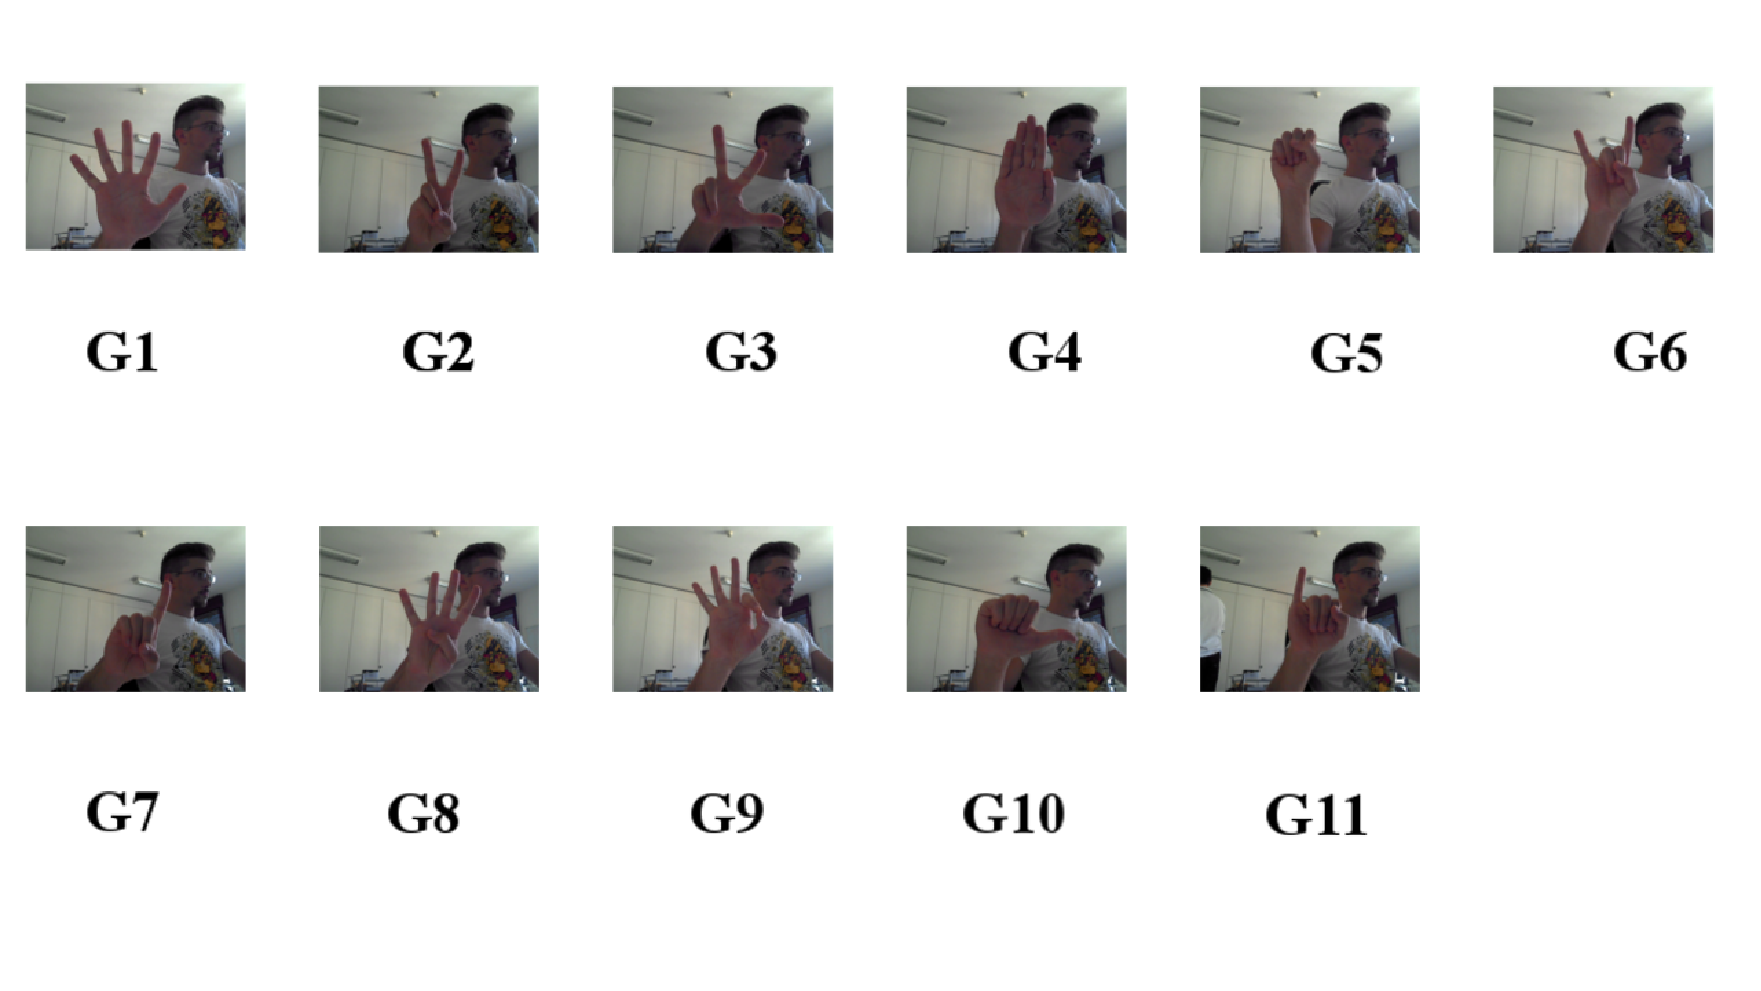
\includegraphics[width=%
1\textwidth]{figures/Gesti}
\caption[Immagini RGB degli 11 gesti.]{Rappresentazione degli 11 gesti prendendo per ciascuno una delle 30 immagini RGB disponibili nel dataset relative alla prima persona.
\label{fig:undicigesti}}
\end{figure}

Il lavoro proposto si compone di una fase iniziale di elaborazione dei dati di input. Ogni file viene letto e risalvato in formato NPY, poichè la rete neurale accetta in ingresso dati di questo formato. Un file NPY è un file di array NumPy creato dal pacchetto software di Python tramite la libreria NumPy. Esso contiene un array salvato nel formato di file NumPy (NPY), inoltre i file NPY memorizzano tutte le informazioni necessarie per ricostruire un array su qualsiasi computer, che include le informazioni su dtype e forma.
Inizialmente è creato un ulteriore array di target che serve durante la fase di allenamento, ad esso, per ogni file NPY, sarà aggiunto il valore da 1 a 11 corrispondente al gesto che viene rappresentato.

Inoltre qui avviene la prima elaborazione dei dati di input, i quali vengono "puliti", riscalati e filtrati. Non ci si è soffermati sulla pulizia che consiste in una semplice rimozione dello sfondo, ad esempio tutti i campioni che rappresentano lo sfondo dell'immagine vengono impostati a zero mentre si lasciano invariati i numeri che descrivono il gesto della mano.
Per la mappa di profondità viene utilizzato un filtro mediano. Questa funzione prende la mediana di tutti i pixel sotto l'area del kernel e l'elemento centrale viene sostituito dalla mediana nella finestra. Nella sfocatura mediana, l'elemento centrale viene sempre sostituito da qualche valore di pixel nell'immagine, in tal modo riesce a ridurre efficacemente il rumore impulsivo.
Sono illustrati in Figura \textbf{\ref{fig:vettorenpy}} alcuni gesti presi dai file in formato NPY e che quindi hanno già subito tutto il processo di elaborazione (nell'immagine essi sono già stati anche normalizzati).

\begin{figure}
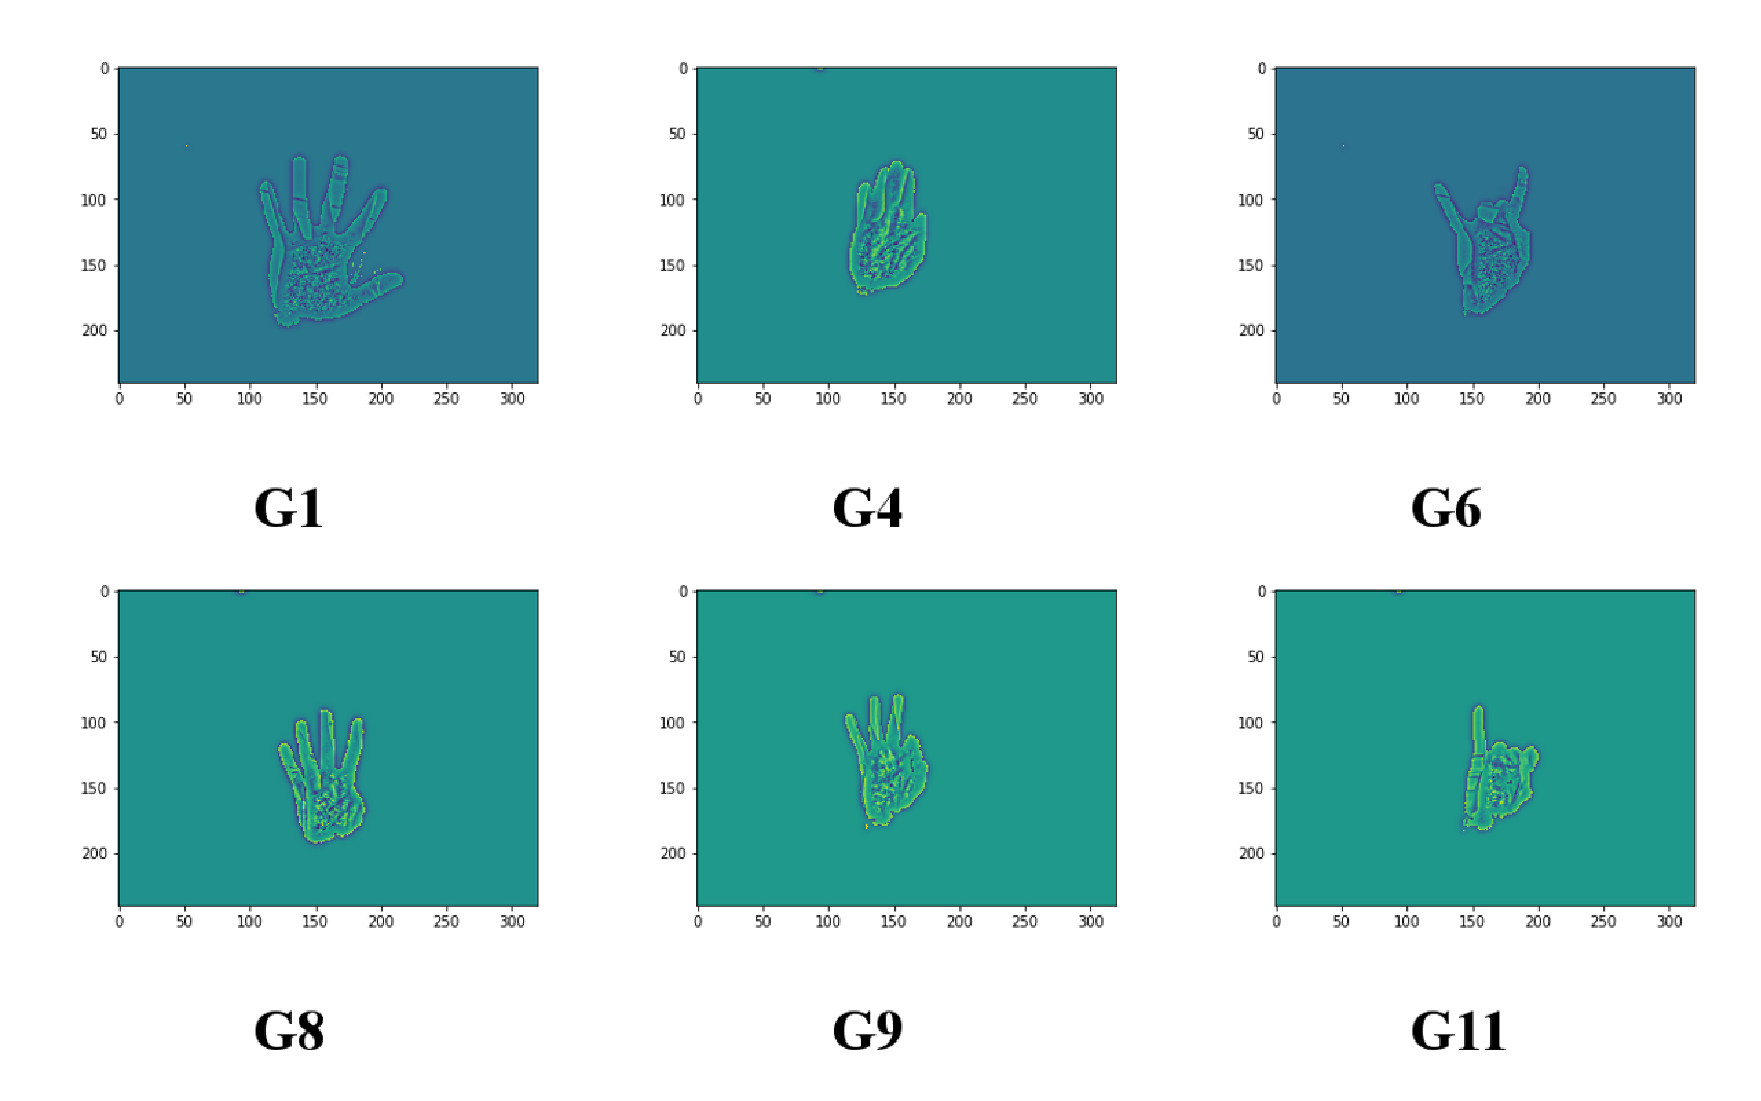
\includegraphics[width=%
1\textwidth]{figures/GestiNpy}
\caption[Vettore NPY di alcuni gesti.]{Rappresentazione grafica di vettori NPY in 2D di alcuni gesti, poco prima di essere elaborati dalla rete neurale.
\label{fig:vettorenpy}}
\end{figure}

Questi file NPY successivamente vengono inviati alla rete neurale convoluzionale. La rete prende in input i file e produce un vettore di classificazione usando quattro strati convoluzionali di risoluzione progressivamente ridotta. I vari vettori di classificazione sono finalmente elaborati da un classificatore lineare che %combina le uscite dei vari rami e
produce l'output finale. Questo è il funzionamento in generale, successivamente sarà spiegato nello specifico in quanto ci sono alcune variazioni in base all'approccio che viene scelto.
Per la conclusione del paragrafo è mostrato un frammento del codice riguardante il filtraggio, la scalatura e la pulizia dei file (per quest'ultima è stato scelto un valore di soglia fisso di 400).\\

\textbf{Codice:} Esempio di elaborazione dei file di input. 
\begin{python}

depth=np.load(os.path.join(inpt_dir,'trainsource', id+'.npy'))
conf=np.load(os.path.join(inpt_dir,'trainsourceConf', id+'.npy'))
img=np.load(os.path.join(inpt_dir,'trainsourceColorRGB', id+'.npy'))
        
depth=cv2.medianBlur(depth,5)
imgR=pc.resize(img[:,:,0],(240,320),'linear').astype('float32')
imgG=pc.resize(img[:,:,1],(240,320),'linear').astype('float32')
imgB=pc.resize(img[:,:,2],(240,320),'linear').astype('float32')

for k in range(len(conf[0,:,:])):
    for q in range(len(conf[0,k,:])):
        if(conf[0,k,q] < 400):
	 conf[0,k,q]= 0
            depth[0,k,q]=0
            conf[0,k,q]=0
            imgR[k,q]=0
            imgG[k,q]=0
            imgB[k,q]=0
\end{python}